\documentclass[a4paper,10pt,twoside,twocolumn]{dndbook} %a4, 10pt, book (idk why i did that...), 2 cols, dnd-themed
\usepackage[english]{babel} %language
\usepackage[utf8]{inputenc} %lovely utf-8
\usepackage{graphicx} %images
\usepackage{wrapfig} %images
\usepackage{array} %allways use this shit, idk why
\usepackage{tikz} %draw stuff
\usepackage{ifthen} %draw stuff
\usetikzlibrary{shapes,calc,fadings} %draw stuff
\usepackage{xspace} %usefull idk, allways import this stuff
\usepackage{dirtytalk} %\say because fuck it
\usepackage{setspace} %don't ask, kind of like it...
\usepackage{pgfplots}

\usepackage[singlelinecheck=false]{caption} %idk dndbook...
\usepackage{listings} %idk dndbook...
\usepackage{shortvrb} %not used yet...
\usepackage{stfloats} %idk dndbook

%5 pages

\singlespacing
\makeatletter %because of titlepage and \HUGE

\def \license {GNU Free Documentation License (https://www.gnu.org/licenses/fdl-1.3)}
\def \author {Sven Hugi}%if you edit this document, add your name... <3

%highlighting with some random effect -> looks handmade and i love it...
\newcommand\hl[2][yellow]{
	\begin{tikzpicture}[
	baseline,
	decoration={random steps,amplitude=1pt,segment length=15pt},
	outer sep=-15pt, inner sep = 0pt
	]
	\node[decorate,rectangle,fill=#1,anchor=text]{#2\xspace};
	\end{tikzpicture}
}
%2 column layout hack...
\newcommand{\nextPage}{
	\newpage
	\hbox{}
	\newpage
}
%the old HUGE fontsize
\newcommand\HUGE{\@setfontsize\Huge{60}{80}} 

\renewcommand{\maketitle}{
	\pagestyle{empty}
	\onecolumn %fuck it
	\vspace*{5cm}
	\begin{center}
		$\vspace*{2cm}$
		{\Huge
			{\HUGE\DndFontDropCap{D}}{\Huge$^{\&}$}{\HUGE\DndFontDropCap{D}}
			\\{5e}\\DM-Screen\\W20 Special\\
		}	
	\end{center}
	\vfill
	Author(s):\linebreak$\vspace{0.3cm}$\author\linebreak
	Licenses\linebreak$\vspace{0.4cm}$\license\linebreak
	\section*{\tiny \hfill Document written in \LaTeX}
}\makeatother
%%%%%%%%%%%%%%%%%%%%%%%%%%%%%%%%%%%%%%%%%%%%%%%%%%%%%%%%%%%%%%%%%%%%%%%%%%%%%%%%%%%%%%%%%%%%%%%%%%%%%%%%%%%%%%%%%%%%%%%%%%%%%%%%%
%											Begin with the fucking document														%
%%%%%%%%%%%%%%%%%%%%%%%%%%%%%%%%%%%%%%%%%%%%%%%%%%%%%%%%%%%%%%%%%%%%%%%%%%%%%%%%%%%%%%%%%%%%%%%%%%%%%%%%%%%%%%%%%%%%%%%%%%%%%%%%%
\begin{document}
	\maketitle
	\twocolumn %reset shit
	\thispagestyle{empty}%no footer
	%\section{Combat}
	\begin{DndSidebar}{Actions in Comba}
		\textbf{Attack}\linebreak
		You make a melee or ranged weapon attack.\linebreak
		\textbf{Cast a Spell}\linebreak
		You cast a cantrip or spell of 1st level or higher. See the spell's casting time.\linebreak
		\textbf{Dash}\linebreak
		You gain extra movement equal to your speed (plus any modifiers) for the current turn.\linebreak
		\textbf{Disengage}\linebreak
		Your movement doesn't provoke opportunity attacks for the rest of the turn.\linebreak
		\textbf{Dodge}\linebreak
		When you take the Dodge action, you focus entirely on avoiding attacks. Until the start of your next turn, any attack roll made against you has disadvantage if you can see the attacker, and you make Dexterity saving throws with advantage. You lose this benefit if you are incapacitated or if your speed drops to 0. \linebreak
		\textbf{Help}\linebreak
		When you take the Help action, the creature you aid gains advantage on the next ability check it makes to perform the task you are helping with.
		Alternatively, you can distract one creature within 5 feet of you, and the next attack roll that an ally of yours makes against that creature has advantage. Whichever option your choose, the advantage goes away once used or when your next turn starts.\linebreak
		\textbf{Hide}\linebreak
		You make a Dexterity (Stealth) check in an attemp to become hidden $\rightarrow$ unseen and unheard.\linebreak
		\textbf{Ready}\linebreak
		You wait for a particular circumstance befor you act, which lets you act using your reaction before the start of your next turn. You must deside in advance (a) what percivable circumstance will trigger your reaction and (b) the action you will take on response to that trigger. If you ready a spell, it must have a casting time of 1 action, and you must concentrate on it until you release it.\linebreak
		\textbf{Search}\linebreak
		You make a Wisdom (Perception) or an Intelligence (Investigation) check to find something.\linebreak
		\textbf{Use a Magic Item}\linebreak
		You use a magic item that requires your action for its use.\linebreak
		\textbf{Use an Object}\linebreak
		You use an object, other than a magic item, that requires your action for its use.\linebreak
		\textbf{Use a Special Ability}\linebreak
		You use a class feature or other special ability that requires your action for its use.\linebreak
	\end{DndSidebar}
	\begin{DndSidebar}{Things You Can Do on Your Turn}
		\begin{itemize}
			\item Move up to your speed.
			\item Take one Action.
			\item Communicate with speech, gestures, or both.
			\item Interact with one object or feature of the environment as you move or take your action. To interact with a second object, take the Use an Object action.
		\end{itemize}
	\end{DndSidebar}
	\begin{DndSidebar}{Spells}
		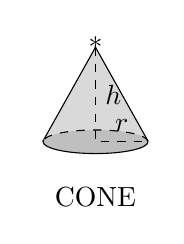
\begin{tikzpicture}
			\newcommand{\radiusx}{2}%gets devided by 3 because 0.x is not allowed in some random stuff... idk fix it...
			\newcommand{\radiusy}{.15}
			\newcommand{\height}{1.2}
			
			\coordinate (a) at (-{\radiusx/3*sqrt(1-(\radiusy/\height)*(\radiusy/\height))},{\radiusy*(\radiusy/\height)});
			\coordinate (b) at ({\radiusx/3*sqrt(1-(\radiusy/\height)*(\radiusy/\height))},{\radiusy*(\radiusy/\height)});
			
			\draw[fill=gray!30] (a)--(0,\height)--(b)--cycle;
			
			\fill[gray!50] circle (\radiusx{}/3 and \radiusy);
			
			\begin{scope}
			\clip ([xshift=-2mm]a) rectangle ($(b)+(1mm,-2*\radiusy)$);
			\draw circle (\radiusx{}/3 and \radiusy);
			\end{scope}
			
			\begin{scope}
			\clip ([xshift=-2mm]a) rectangle ($(b)+(1mm,2*\radiusy)$);
			\draw[dashed] circle (\radiusx{}/3 and \radiusy);
			\end{scope}
			
			\draw[dashed] (0,\height)|-(\radiusx/3,0) node[right, pos=.25]{$h$} node[above,pos=.75]{$r$};
			
			\node at (0, -0.7){CONE};
			\node at (0, \height){*};
		
		\end{tikzpicture}
		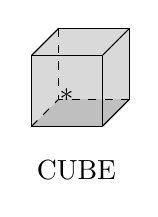
\begin{tikzpicture}
			%a other way:
			%\draw[yslant=-0.5] (0,0) grid (1,1);
			%\draw[yslant=-0.5, dashed] (1,2) -- (1,1);
			%\draw[yslant=-0.5, dashed] (2,1) -- (1,1);
			%\draw[yslant=-0.5, dashed] (0,0) -- (1,1);
			%\draw[yslant=0.5] (1,-1) grid (2,0);
			%\draw[yslant=0.5,xslant=-1] (1,0) grid (2,1);
			
			\newcommand{\Depth}{0.9}
			\newcommand{\Height}{0.9}
			\newcommand{\Width}{0.9}
			
			\coordinate (O) at (0,0,0);
			\coordinate (A) at (0,\Width,0);
			\coordinate (B) at (0,\Width,\Height);
			\coordinate (C) at (0,0,\Height);
			\coordinate (D) at (\Depth,0,0);
			\coordinate (E) at (\Depth,\Width,0);
			\coordinate (F) at (\Depth,\Width,\Height);
			\coordinate (G) at (\Depth,0,\Height);
			
			\fill[gray!30] (O) -- (A) -- (E) -- (D);% Back Face
			\fill[gray!30] (O) -- (A) -- (B) -- (C);% Left Face
			\fill[gray!30] (D) -- (E) -- (F) -- (G);% Right Face
			\fill[gray!50] (O) -- (C) -- (G) -- (D);% Bottom Face
			
			\draw [dashed] (C) -- (O);
			\draw [dashed] (D) -- (O);
			\draw [dashed] (A) -- (O);
			\draw (A) -- (E);
			\draw (D) -- (G);
			\draw (D) -- (E);
			\draw (E) -- (F);
			\draw (F) -- (G);
			\draw (C) -- (B);
			\draw (B) -- (F);
			\draw (G) -- (C);
			\draw (A) -- (B);
			
			\node at (\Width/4, -\Height){CUBE};
			\node at (0.1, 0){*};
		\end{tikzpicture}
		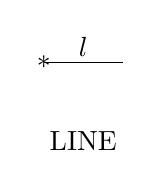
\begin{tikzpicture}
			\draw (0,0) -- (1,0);
			\node at (0, -0.05){*};
			\node at (.5, .2){$l$};
			\node at (0.5, -1){LINE};
		\end{tikzpicture}
		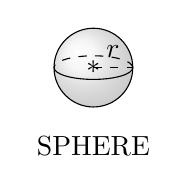
\begin{tikzpicture}
			\shade[ball color = gray!30, opacity = 0.3] (0,0) circle (0.5cm);
			
			\draw (0,0) circle (.5cm);
			\draw (-0.5,0) arc (180:360:0.5 and 0.15);
			\draw[dashed] (0.5,0) arc (0:180:0.5 and 0.15);
			\draw[dashed] (0,0) -- node[above]{$r$} (0.5,0);
			
			\node at (0, -1){SPHERE};
			\node at (0, -0.05){*};
		\end{tikzpicture}
		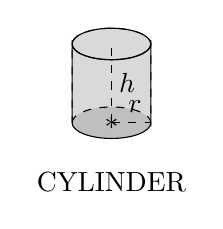
\begin{tikzpicture}    
			\coordinate (ll) at (-0.5,-0.5);
			\coordinate (lr) at (0.5,-0.5);
			\coordinate (ul) at (-0.5,0.5);
			\coordinate (ur) at (0.5,0.5);
			
			\fill [gray!50] (ll) arc (-180:0:0.5cm and .2cm) -- (ur) arc (0:-180:0.5cm and .2cm) -- cycle;
			\fill [gray!30]  (ll) arc (180:0:0.5cm and .2cm)-- (ur) arc (0:180:0.5cm and .2cm) -- cycle;
			
			\draw (ll) arc (-180:0:0.5cm and .2cm) -- (ur) arc (0:-180:0.5cm and .2cm) -- cycle;
			\draw [dashed] (ll) arc (180:0:0.5cm and .2cm) -- (ur) arc (0:180:0.5cm and .2cm) -- cycle;
			\draw (ul) arc (-180:180:0.5cm and .2cm);
			\draw [dashed] (0,-0.5) -- (0,0.5);
			\draw[dashed] (0,-0.5) -- (0.5,-0.5);
			
			\node at (0,-.55){*};
			\node at (0.3, -.3) {$r$};
			\node at (0.2, 0) {$h$};
			\node at (0, -1.25){CYLINDER};
		\end{tikzpicture}
		\begin{center}
			* Point of origin
		\end{center}
	\end{DndSidebar}
	\pagebreak
	%\section{Moving}
	\begin{DndSidebar}{Jumping}
		\textbf{Long Jump}\linebreak
		When you make a long jump, you cover a number of feet up to your Strength score if you move at least 10 feet on foot immediately before the jump. When you make a standing long jump, you can leap only half that distance.\linebreak
		\textbf{High Jump}\linebreak
		When you make a high jump, you leap into the air a number of feet equal to 3 + your Strength modifier if you move at least 10 feet on foot immediately before the jump. When you make a standing high jump, you can jump only half that distance.\linebreak
	\end{DndSidebar}
	\begin{DndSidebar}{Traveling}
		\textbf{Forced March}\linebreak
		The Travel Pace table assumes that characters travel for 8 hours in day. They can push on beyond that limit, at the risk of exhaustion.
		For each additional hour of travel beyond 8 hours, the characters cover the distance shown in the Hour column for their pace, and each character must make a Constitution saving throw at the end of the hour. The DC is 10 + 1 for each hour past 8 hours. On a failed saving throw, a character suffers one level of exhaustion.\linebreak
		\textbf{Mounts and Vehicles}\linebreak
		A mounted character can ride at a gallop for about an hour, covering twice the usual distance for a fast pace. If fresh mounts are available every 8 to 10 miles, characters can cover larger distances at this pace, but this is very rare except in densely populated areas. Characters in wagons, carriages, or other land vehicles choose a pace as normal. Characters in a waterborne vessel are limited to the speed of the vessel, and they don't suffer penalties for a fast pace or gain benefits from a slow pace. Depending on the vessel and the size of the crew, ships might be able to travel for up to 24 hours per day.
		Certain special mounts, such as a pegasus or griffon, or special vehicles, such as a carpet of flying, allow you to travel more swiftly.\linebreak
	\end{DndSidebar}
	\begin{DndTable}[header=Travel Pace]{llllX}
		\textbf{Pace}	&\textbf{Minute}	&\textbf{Hour}	&\textbf{Day}	&\textbf{Effect}\\
		Fast 			&$400 ft$			&$4 mi$			&$30 mi$		&-$5$ penalty to passive Wisdom (Perception) scores\\
		Normal			&$300 ft$			&$3 mi$			&$24 mi$		&\\
		Slow			&$200 ft$			&$2 mi$			&$18 mi$		&Able to use stealth
	\end{DndTable}
	\begin{DndSidebar}{Climbing, Swimming, and Crawling}
		While climbing or swimming, each foot of movement costs 1 extra foot (2 extra feet in difficult terrain), unless a creature has a climbing or swimming speed. At the GM’s option, climbing a slippery vertical surface or one with few handholds requires a successful Strength (Athletics) check. Similarly, gaining any distance in rough water might require a successful Strength (Athletics) check. 
	\end{DndSidebar}
	\begin{DndSidebar}{Difficult Terrain}
		Adventurers often face dense forests, deep swamps, rubble-filled ruins, steep mountains, and ice-covered ground, all considered difficult terrain. You move at half speed in difficult terrain $\rightarrow$ moving 1 foot in difficult terrain costs 2 feet of speed, so you can cover only half the normal distance in a minute, an hour, or a day. 
	\end{DndSidebar}
	\pagebreak
	\section{Conditions}
	\begingroup
	\DndSetThemeColor[DmgCoral]
	\begin{DndSidebar}{Warning}
		\textbf{Conditions can really suck!}\linebreak
		Don't use them to often.
	\end{DndSidebar}
	\endgroup
	\begin{DndSidebar}{}
		\textbf{Blinded}
		\begin{itemize}
			\item A blinded creature can't see and automatically fails any ability check that requires sight.
			\item Attack rolls against the creature have advantage, and the creature's attack rolls have disadvantage. 
		\end{itemize}
	\textbf{Charmed}
	\begin{itemize}
		\item A charmed creature can't attack the charmer or target the charmer with harmful abilities or magical effects.
		\item The charmer has advantage on any ability check to interact socially with the creature.
	\end{itemize}
	\textbf{Deafened}
	\begin{itemize}
		\item A deafened creature can't hear and automatically fails any ability check that requires hearing.
	\end{itemize}
	\textbf{Frightened}
	\begin{itemize}
		\item A frightened creature has disadvantage on ability checks and attack rolls while the source of its fear is within line of sight.
		\item The creature can't willingly move closer to the source of its fear.
	\end{itemize}
	\textbf{Grappled}
	\begin{itemize}
		\item A grappled creature's speed becomes 0, and it can't benefit from any bonus to its speed.
		\item The condition ends if the grappler is incapacitated (see the condition).
		\item The condition also ends if an effect removes the grappled creature from the reach of the grappler or grappling effect, such as when a creature is hurled away by the thunder-wave spell.
	\end{itemize}
	\textbf{Incapacitated}
	\begin{itemize}
		\item An incapacitated creature can't take actions or reactions. 
	\end{itemize}
	\textbf{Invisible}
	\begin{itemize}
		\item An invisible creature is impossible to see without the aid of magic or a special sense. For the purpose of hiding, the creature is heavily obscured. The creature's location can be detected by any noise it makes or any tracks it leaves.
		\item Attack rolls against the creature have disadvantage, and the creature's attack rolls have advantage.
	\end{itemize}
	\textbf{Paralyzed}
	\begin{itemize}
		\item A paralyzed creature is incapacitated (see the condition) and can't move or speak.
		\item The creature automatically fails Strength and Dexterity saving throws. Attack rolls against the creature have advantage.
		\item Any attack that hits the creature is a critical hit if the attacker is within 5 feet of the creature.
	\end{itemize}
	\textbf{Petrified}
	\begin{itemize}
		\item A petrified creature is transformed, along with any nonmagical object it is wearing or carrying, into a solid inanimate substance (usually stone). Its weight increases by a factor of ten, and it ceases aging.
		\item The creature is incapacitated (see the condition), can't move or speak, and is unaware of its surroundings.
		\item Attack rolls against the creature have advantage.
		\item The creature automatically fails Strength and Dexterity saving throws.
		\item The creature has resistance to all damage.
		\item The creature is immune to poison and disease.
	\end{itemize}
	\textbf{Poisoned}
	\begin{itemize}
		\item A poisoned creature has disadvantage on attack rolls and ability checks.
	\end{itemize}
	\end{DndSidebar}
	\begin{DndSidebar}{}
	\textbf{Prone}
	\begin{itemize}
		\item A prone creature's only movement option is to crawl, unless it stands up and thereby ends the condition.
		\item The creature has disadvantage on attack rolls.
		\item An attack roll against the creature has advantage if the attacker is within 5 feet of the creature. Otherwise, the attack roll has disadvantage.
	\end{itemize}
	\textbf{Restrained}
	\begin{itemize}
		\item A restrained creature's speed becomes 0, and it can't benefit from any bonus to its speed.
		\item Attack rolls against the creature have advantage, and the creature's attack rolls have disadvantage.
		\item The creature has disadvantage on Dexterity saving throws.
	\end{itemize}
	\textbf{Stunned}
	\begin{itemize}
		\item A stunned creature is incapacitated (see the condition), can't move, and can speak only falteringly.
		\item The creature automatically fails Strength and Dexterity saving throws.
		\item Attack rolls against the creature have advantage.
	\end{itemize}
	\textbf{Unconscious}
	\begin{itemize}
		\item An unconscious creature is incapacitated (see the condition), can't move or speak, and is unaware of its surroundings
		\item The creature drops whatever it's holding and falls prone.
		\item The creature automatically fails Strength and Dexterity saving throws.
		\item Attack rolls against the creature have advantage.
		\item Any attack that hits the creature is a critical hit if the attacker is within 5 feet of the creature.
	\end{itemize}
	\textbf{Exhaustion}\linebreak
	Some special abilities and environmental hazards, such as starvation and the long-term effects of freezing or scorching temperatures, can lead to a special condition called exhaustion. An effect can give a creature one or more levels of exhaustion, as specified in the effect's description. A creature suffers the effect of its current level of exhaustion as well as all lower levels. Finishing a long rest reduces a creature's exhaustion level by 1, provided that the creature has also ingested some food and drink. 
	\end{DndSidebar}
	\begin{DndTable}[header=Exhaustion]{lX}
		\textbf{Level} & \textbf{Effect}\\
		$1$	&Disadvantage on ability checks\\
		$2$	&Speed halved\\
		$3$	&Disadvantage on attack rolls and saving throws\\
		$4$	&Hit point maximum halved\\
		$5$	&Speed reduced to $0$\\
		$6$	&Death\\
	\end{DndTable}
	\begin{DndSidebar}{Food and Water}
		\textbf{Food}\linebreak
		A character can go without food for a number of days equal to 3 + his or her Constitution modifier (minimum 1). At the end of each day beyond that limit, a character automatically suffers one level of exhaustion.\linebreak
		\textbf{Water}\linebreak
		A character needs one gallon of water per day, or two gallons per day if the weather is hot. A character who drinks only half that much water must succeed on a DC 15 Constitution saving throw or suffer one level of exhaustion at the end of the day. A character with access to even less water automatically suffers one level of exhaustion at the end of the day. If the character already has one or more levels of exhaustion, the character takes two levels in either case.
	\end{DndSidebar}
	\pagebreak
	\section{Equipment}
		\begin{DndTable}[header=Coins]{lrrrrr}
		\textbf{Coin}	&\textbf{cp}	&\textbf{sp}	&\textbf{ep}	&\textbf{gp}	&\textbf{pp}\\
		\textbf{cp}		&$1$			&$\frac{1}{10}$	&$\frac{1}{50}$	&$\frac{1}{100}$&$\frac{1}{1000}$\\
		\textbf{sp}		&$10$			&$1$			&$\frac{1}{5}$	&$\frac{1}{10}$	&$\frac{1}{100}$\\
		\textbf{ep}		&$50$			&$5$			&$1$			&$\frac{1}{2}$	&$\frac{1}{20}$\\
		\textbf{gp}		&$100$			&$10$			&$2$			&$1$			&$\frac{1}{10}$\\
		\textbf{pp}		&$1000$			&$100$			&$20$			&$1$			&$1$\\
	\end{DndTable}
	\begin{DndTable}[header=Armor]{llllX}
		\textbf{Light}	&\textbf{Cost}	&\textbf{AC}		&\textbf{STR}	&\textbf{Stealth}\\
		Padded			&$5$ gp			&$11$ + Dex			&				&$D$\\
		Leather			&$10$ gp		&$11$ + Dex			&				&\\
		Studded leather	&$45$ gp		&$12$ + Dex			&				&\\
		\textbf{Medium}	&\textbf{Cost}	&\textbf{AC}		&\textbf{STR}	&\textbf{Stealth}\\
		Hide			&$10$ gp 		&$12$ + Dex ($2$)	&				&\\
		Chain shirt		&$50$ gp		&$13$ + Dex ($2$)	&				&\\
		Scale mail		&$50$ gp		&$14$ + Dex ($2$)	&				&$D$\\
		Breastplate		&$400$ gp		&$14$ + Dex ($2$)	&				&\\
		Half plate		&$750$ gp		&$15$ + Dex ($2$)	&				&$D$\\
		\textbf{Heavy}	&\textbf{Cost}	&\textbf{AC}		&\textbf{STR}	&\textbf{Stealth}\\
		Ring mail		&$30$ gp		&$14$				&				&$D$\\
		Chain mail		&$75$ gp		&$16$				&$13$			&$D$\\
		Splint			&$200$ gp		&$17$				&$15$			&$D$\\
		Plate			&$1500$ gp		&$18$				&$15$			&$D$\\
		\textbf{Shield}	&\textbf{Cost}	&\textbf{AC}		&\textbf{STR}	&\textbf{Stealth}\\
		Shield			&$10$ gp		&+$2$				&				&
	\end{DndTable}
	\begin{DndSidebar}{Getting Into and Out of Armor}
		The time it takes to don or doff armor depends on the armor's category.\linebreak
		\textbf{Don}. This is the time it takes to put on armor. You benefit from the armor's AC only if you take the full time to don the suit of armor.\linebreak
		\textbf{Doff}. This is the time it takes to take off armor. If you have help, reduce this time by half.
	\end{DndSidebar}
	\begin{DndTable}[header=Don and Doff]{lll}
		\textbf{Category}	&\textbf{Don}	&\textbf{Doff}\\
		Light Armor			&$1$ min		&$1$ min\\
		Medium Armor		&$5$ min		&$1$ min\\
		Heavy Armor			&$10$ min		&$5$ min\\
		Shield				&$1$ action		&$1$ action\\
	\end{DndTable}
	\begin{DndTable}[header=Simple Melee Weapons]{lllX}
		\textbf{Type}	&\textbf{Cost}	&\textbf{Damage}	 	&\textbf{Properties}\\
		Club			&$1$ sp			&$1$d$4$ Bludgeoning	&Light\\
		Dagger			&$2$ gp			&$1$d$4$ Piercing		&Finesse, Light, Thrown($20/60$)\\
		Greatclub 		&$2$ sp			&$1$d$8$ Bludgeoning	&Two-handed\\
		Handaxe 		&$5$ gp			&$1$d$6$ Slashing 		&Light, Thrown ($20/60$)\\
		Javelin 		&$5$ sp			&$1$d$6$ Piercing		&Thrown ($30/120$)\\
		Light hammer 	&$2$ gp			&$1$d$4$ Bludgeoning	&Light, Thrown ($20/60$)\\
		Mace 			&$5$ gp			&$1$d$6$ Bludgeoning	&\\
		Quarterstaff 	&$2$ gp			&$1$d$6$ Bludgeoning	&Versatile ($1$d$8$)\\
		Sickle 			&$1$ gp			&$1$d$4$ Slashing		&Light\\
		Spear 			&$1$ gp			&$1$d$6$ Piercing	 	&Thrown ($20/60$), Versatile ($1$d$8$)\\
	\end{DndTable}
	\begin{DndTable}[header=Simple Ranged Weapons]{lllX}
		\textbf{Type}	&\textbf{Cost}	&\textbf{Damage}	 	&\textbf{Properties}\\
		Crossbow, light &$25$ gp		&$1$d$8$ Piercing		&Ammunition ($80/320$), Loading, Two-handed\\
		Dart 			&$5$ cp			&$1$d$4$ Piercing 		&Finesse, Thrown ($20/60$)\\
		Shortbow 		&$25$ gp		&$1$d$6$ Piercing		&Ammunition ($80/320$), Two-handed\\
		Sling 			&$1$ sp			&$1$d$4$ Bludgeoning	&Ammunition ($30/120$)\\
	\end{DndTable}
	\begin{DndTable}[header=Martial Melee Weapons]{lllX}
		\textbf{Type}	&\textbf{Cost}	&\textbf{Damage}	 	&\textbf{Properties}\\
		Battleaxe 		&$10$ gp		&$1$d$8$ Slashing		&Versatile ($1$d$10$)\\
		Flail 			&$10$ gp		&$1$d$8$ Bludgeoning	&\\
		Glaive 			&$20$ gp		&$1$d$10$ Slashing		&Heavy, Reach, Two-handed\\
		Greataxe 		&$30$ gp		&$1$d$12$ Slashing		&Heavy, Two-handed\\
		Greatsword 		&$50$ gp		&$2$d$6$ Slashing		&Heavy, Two-handed\\
		Halberd 		&$20$ gp		&$1$d$10$ Slashing		&Heavy, Reach, Two-handed\\
		Lance			&$10$ gp		&$1$d$12$ Piercing		&Reach, Special\\
		Longsword		&$15$ gp		&$1$d$8$ Slashing		&Versatile ($1$d$10$)\\
		Maul			&$10$ gp		&$2$d$6$ Bludgeoning	&Heavy, Two-handed\\
		Morningstar 	&$15$ gp		&$1$d$8$ Piercing		&\\
		Pike 			&$5$ gp 		&$1$d$10$ Piercing		&Heavy, Reach, Two-handed\\
		Rapier 			&$25$ gp 		&$1$d$8$ Piercing 		&Finesse\\
		Scimitar 		&$25$ gp 		&$1$d$6$ Slashing 		&Finesse, Light\\
		Shortsword 		&$10$ gp 		&$1$d$6$ Piercing 		&Finesse, Light\\
		Trident 		&$5$ gp 		&$1$d$6$ Piercing 		&Thrown ($20/60$), versatile ($1$d$8$)\\
		War pick 		&$5$ gp			&$1$d$8$ Piercing		&\\
		Warhammer 		&$15$ gp 		&$1$d$8$ Bludgeoning	&Versatile ($1$d$10$)\\
		Whip 			&$2$ gp			&$1$d$4$ Slashing		&Finesse, Reach\\
	\end{DndTable}
	\begin{DndTable}[header=Martial Ranged Weapons]{lllX}
		\textbf{Type}	&\textbf{Cost}	&\textbf{Damage}	 	&\textbf{Properties}\\
		Blowgun 		&$10$ gp		&$1$ Piercing			&Ammunition ($25/100$), Loading\\
		Crossbow, hand 	&$75$ gp 		&$1$d$6$ Piercing		&Ammunition ($30/120$), Light, Loading\\
		Crossbow, heavy &$50$ gp 		&$1$d$10$ Piercing		&Ammunition ($100/400$), Heavy, Loading, Two-handed\\
		Longbow 		&$50$ gp 		&$1$d$8$ Piercing 		&Ammunition ($150/600$), Heavy, Two-handed\\
		Net 			&$1$ gp			&						&Special, Thrown ($5/15$)\\
	\end{DndTable}
	\begin{DndTable}[header=Container Capacity]{lX}
		\textbf{Container}	&\textbf{Capacity}\\
		Backpack			&$1$ cubic foot/$30$ pounds of gear\\
		Barrel				&$40$ gallons liquid, $4$ cubic feet solid\\
		Basket 				&$2$ cubic feet/$40$ pounds of gear\\
		Bottle				&$1\frac{1}{2}$ pints liquid\\
		Bucket				&$3$ gallons liquid/$\frac{1}{2}$ cubic foot solid\\
		Chest				&$12$ cubic feet/$300$ pounds gear\\
		Flask or tankard	&$1$ pint liquid\\
		Jug or pitcher		&$1$ gallon liquid\\
		Pot, iron			&$1$ gallon liquid\\
		Pouch				&$\frac{1}{5}$ cubic foot/$6$ pounds of gear\\
		Sack				&$1$ cubic foot/$30$ pounds of gear\\
		Vial				&$4$ ounces liquid\\
		Waterskin			&$4$ pints liquid\\
	\end{DndTable}
	\begin{DndTable}[header=Mounts]{lllX}
		\textbf{Item}	&\textbf{Cost}	&\textbf{Speed}	&\textbf{Carrying Capacity}\\
		Camel			&$50$ gp		&$50 ft$		&$480 lb$\\
		Donkey or mule	&$8$ gp			&$40 ft$		&$420 lb$\\
		Elephant		&$200$ gp		&$40 ft$		&$1,320 lb$\\
		Horse, draft	&$50$ gp		&$40 ft$		&$540 lb$\\
		Horse, riding	&$75$ gp		&$60 ft$		&$480 lb$\\
		Mastiff			&$25$ gp		&$40 ft$		&$195 lb$\\
		Pony			&$30$ gp		&$40 ft$		&$225 lb$\\
		Warhorse		&$400$ gp		&$60 ft$		&$40 lb$\\
	\end{DndTable}
	\begin{DndTable}[header=Tack Harness and Drawn Vehicles]{llX}
		\textbf{Item}		&\textbf{Cost}	&\textbf{Weight}\\
		Barding				&$x4$			&$x2$\\
		Bit and bridle		&$2$ gp			&$1 lb$\\
		Carriage			&$100$ gp		&$600 lb$\\
		Cart				&$15$ gp		&$200 lb$\\
		Chariot				&$250$ gp		&$100 lb$\\
		Feed (per day)		&$5$ cp			&$10 lb$\\
		Saddlebags			&$4$ gp			&$8 lb$\\
		Sled				&$20$ gp		&$300 lb$\\
		Stabling (per day)	&$5$ sp 		&\\
		Wagon				&$35$ gp		&$400 lb$\\
	\end{DndTable}
	\begin{DndSidebar}{Torch}
		A torch burns for 1 hour, providing bright light in a 20-foot radius and dim light for an additional 20 feet. If you make a melee attack with a burning torch and hit, it deals 1 fire damage.
	\end{DndSidebar}
	\begin{DndTable}[header=Saddles]{lll}
		\textbf{Item}	&\textbf{Cost}	&\textbf{Weight}\\
		Exotic			&$60$ gp		&$40 lb$\\
		Military		&$20$ gp		&$30 lb$\\
		Pack			&$5$ gp			&$15 lb$\\
		Riding			&$10$ gp		&$25 lb$\\
	\end{DndTable}
	\begin{DndTable}[header=Waterborne Vehicles]{lll}
		\textbf{Item}	&\textbf{Cost}	&\textbf{Speed}\\
		Galley			&$30,000$ gp	&$4 mph$\\
		Keelboat		&$3,000$ gp		&$1 mph$\\
		Longship		&$10,000$ gp	&$3 mph$\\
		Rowboat			&$50$ gp		&$1 \frac{1}{2} mph$\\
		Sailingship		&$10,000$ gp	&$2 mph$\\
		Warship			&$25,000$ gp	&$2 \frac{1}{2} mph$\\
	\end{DndTable}
	\begin{minipage}[t]{.18 \textwidth}
	\begin{DndTable}[header=CR to XP]{lX}
		\textbf{CR}		& \textbf{XP}\\
		$0$				&$10$\\
		$\frac{1}{8}$	&$25$\\
		$\frac{1}{4}$	&$50$\\
		$\frac{1}{2}$	&$100$\\
		$1$				&$200$\\
		$2$				&$450$\\
		$3$				&$700$\\
		$4$				&$1,100$\\
		$5$				&$1,800$\\
		$6$				&$2,300$\\
		$7$				&$2,900$\\
		$8$				&$3,900$\\
		$9$				&$5,000$\\
		$10$			&$5,900$\\
		$11$			&$7,200$\\
		$12$			&$8,400$\\
		$13$			&$10,000$\\
		$14$			&$11,500$\\
		$15$			&$13,000$\\
		$16$			&$15,000$\\
		$17$			&$18,000$\\
		$18$			&$20,000$\\
		$19$			&$22,000$\\
		$20$			&$25,000$\\
		$21$			&$33,000$\\
		$22$			&$41,000$\\
		$23$			&$50,000$\\
		$24$			&$62,000$\\
		$25$			&$75,000$\\
		$26$			&$90,000$\\
		$27$			&$150,000$\\
		$28$			&$120,000$\\
		$29$			&$135,000$\\
		$30$			&$155,000$\\
	\end{DndTable}
	\end{minipage}
	\begin{minipage}[t]{.27 \textwidth}
	\begin{DndTable}[header=Level to XP]{llX}
		\textbf{XP}	& \textbf{Level}	&\textbf{Proficiency Bonus}\\
		$0$				&$1$			&+$2$\\
		$300$			&$2$			&+$2$\\
		$900$			&$3$			&+$2$\\
		$2,700$			&$4$			&+$2$\\
		$6,500$			&$5$			&+$3$\\
		$14,000$		&$6$			&+$3$\\
		$23,000$		&$7$			&+$3$\\
		$34,000$		&$8$			&+$3$\\
		$48,000$		&$9$			&+$4$\\
		$64,000$		&$10$			&+$4$\\
		$85,000$		&$11$			&+$4$\\
		$100,000$		&$12$			&+$4$\\
		$120,000$		&$13$			&+$5$\\
		$140,000$		&$14$			&+$5$\\
		$165,000$		&$15$			&+$5$\\
		$195,000$		&$16$			&+$5$\\
		$225,000$		&$17$			&+$6$\\
		$265,000$		&$18$			&+$6$\\
		$305,000$		&$19$			&+$6$\\
		$355,000$		&$20$			&+$6$\\
	\end{DndTable}
	\begin{DndTable}[header=Cover]{lX}
		\textbf{Cover}	&\textbf{Bonus to AC and Dexsave}\\
		\rowcolor{DmgCoral}half cover		&+$2$\\
		three-quarters	&+$5$\\
		\rowcolor{DmgCoral}total cover 	&Can't get attacked directly.\\
	\end{DndTable}
	\end{minipage}
	\section{Spellcasting} 
	\begin{DndSidebar}{Verbal (V)}
		A character who is gagged or in an area of silence, such as one created by the silence spell, can't cast a spell with a verbal component.
	\end{DndSidebar}
	\begin{DndSidebar}{Somatic (S)}
		Spellcasting gestures might include a forceful gesticulation or an intricate set of gestures. If a spell requires a somatic component, the caster must have free use of at least one hand to perform these gestures.
	\end{DndSidebar}
	\begin{DndSidebar}{Material (M)}
		Casting some spells requires particular objects, specified in parentheses in the component entry. A character can use a \textbf{component pouch} or a \textbf{spellcasting focus} in place of the components specified for a spell. But if a cost is indicated for a component, a character must have that specific component before he or she can cast the spell.
		A spellcaster must have a hand free to access a spell's material components or to hold a spellcasting focus but it can be the same hand that he or she uses to perform somatic components. 
	\end{DndSidebar}

	%cover
	%ac of objects
\end{document}